%%%%%%%%%%%%%%%%%%%%%%%%%%%%%%%%%%%%%%%%%%%%%%%%%%%%%%%%%%%%%%%%%%
%%%%%%%% ICML 2015 EXAMPLE LATEX SUBMISSION FILE %%%%%%%%%%%%%%%%%
%%%%%%%%%%%%%%%%%%%%%%%%%%%%%%%%%%%%%%%%%%%%%%%%%%%%%%%%%%%%%%%%%%

% Use the following line _only_ if you're still using LaTeX 2.09.
%\documentstyle[icml2015,epsf,natbib]{article}
% If you rely on Latex2e packages, like most moden people use this:
\documentclass{article}

% use Times
\usepackage{times}
% For figures
\usepackage{graphicx} % more modern

%H
%\usepackage{caption}
%\usepackage{subcaption}

%\usepackage{epsfig} % less modern
%\usepackage{subfigure} 

% For citations
\usepackage{natbib}

% For algorithms
\usepackage{algorithm}
\usepackage{algorithmic}

% As of 2011, we use the hyperref package to produce hyperlinks in the
% resulting PDF.  If this breaks your system, please commend out the
% following usepackage line and replace \usepackage{icml2015} with
% \usepackage[nohyperref]{icml2015} above.
\usepackage{hyperref}

% Packages hyperref and algorithmic misbehave sometimes.  We can fix
% this with the following command.
\newcommand{\theHalgorithm}{\arabic{algorithm}}

\usepackage{amsmath,amsfonts,amssymb,amsthm}

% Employ the following version of the ``usepackage'' statement for
% submitting the draft version of the paper for review.  This will set
% the note in the first column to ``Under review.  Do not distribute.''
\usepackage{icml2015} 

% Employ this version of the ``usepackage'' statement after the paper has
% been accepted, when creating the final version.  This will set the
% note in the first column to ``Proceedings of the...''
%\usepackage[accepted]{icml2015}


% The \icmltitle you define below is probably too long as a header.
% Therefore, a short form for the running title is supplied here:
\icmltitlerunning{Symbolic Gibbs Sampling in Piecewise Algebraic Graphical Models with Nonlinear Deterministic Constraints}

\usepackage{verbatim}
%\usepackage{ntheorem} % framed and list of theorems [standard,framed,thref] \listtheorems{types}		%COMMENTED BY HADI
\usepackage{color}    % color
\newtheorem{theorem}{Theorem}

%OLD
\newcommand{\fix}{\marginpar{FIX}}
\newcommand{\new}{\marginpar{NEW}}
\newcommand{\ind}[1]{\mathbb{I}[#1]}
\newcommand{\inde}{\mathbb{I}}

\newcommand{\var}{v}
\newcommand{\eq}{\leftarrow}

\newcommand{\LB}{\mathit{LB}}
\newcommand{\UB}{\mathit{UB}}

\newcommand{\B}{\mathbb{B}}
\newcommand{\E}{\mathbb{E}}
\newcommand{\I}{\mathbb{I}}
\newcommand{\R}{\mathbb{R}}

\newcommand{\F}{\mathbb{F}}
\renewcommand{\vec}[1]{\mathbf{#1}}

%NEW:
\newcommand{\tuple}[1] {\langle #1 \rangle}
\newcommand{\bvec}[1]{\textbf{#1}}
\newcommand{\indicator}{\mathbb{I}}%{I\!\!I}
\newcommand{\case}[2]{#2 &\text{ if } #1}%{#1 : #2}
\newcommand{\singlecase}[2]{#2 \quad \text{ if } #1}
\newcommand{\otherwise}[1]{#1 &\text{ otherwise}}
\newcommand{\pr}{p}
\newcommand{\nn}{0.16}


\begin{document} 

\twocolumn[
\icmltitle{Symbolic Gibbs Sampling in Piecewise Algebraic Graphical Models with Nonlinear Deterministic Constraints}

% It is OKAY to include author information, even for blind
% submissions: the style file will automatically remove it for you
% unless you've provided the [accepted] option to the icml2015
% package.
\icmlauthor{Your Name}{email@yourdomain.edu}
\icmladdress{Your Fantastic Institute,
            314159 Pi St., Palo Alto, CA 94306 USA}
\icmlauthor{Your CoAuthor's Name}{email@coauthordomain.edu}
\icmladdress{Their Fantastic Institute,
            27182 Exp St., Toronto, ON M6H 2T1 CANADA}

% You may provide any keywords that you 
% find helpful for describing your paper; these are used to populate 
% the "keywords" metadata in the PDF but will not be shown in the document
\icmlkeywords{Deterministic, evidence, relations, constraints, random variables, Symbolic, Analitical, Gibbs sampling}

\vskip 0.3in
]

\begin{abstract}
In many applications of probabilistic reasoning, there are deterministic relationships between
continuous random variables. These relationships create serious problems for approximate or exact inference.
%Such deterministic conditionals create serious problems for exact or approximate inference.
To avoid the complications, algorithms such as \emph{Bayesian inference using Gibbs sampling} (BUGS) simply disallow such dependencies.  
%For example, in BUGS it is impossible to model observed data that is the sum of two random variables. 
There are no known exact or Monte Carlo inference methods that can handle deterministic constraints beyond the limit of linear dependencies.
%Many classes of conjugate distributions %such as \emph{conditional linear Gaussians} 
%can handle linear deterministic conditionals. 
%General purpose full automated inference in the presence of non-linear deterministic constraints, however, is beyond the scope of the existing conjugate solutions and Monte Carlo algorithms.    
In this paper we fill this gap by contributing a novel framework which,
for the first time, carries out inference in models with nonlinear algebraic deterministic constraints. % that are not discussed in the literature so far.
Our second contribution is to provide an effective MCMC inference technique called \emph{Symbolic Gibbs}, based on the insight that in our model, most costly operations required for Gibbs sampling can be accomplished offline and prior to sampling. 
We evaluate this algorithm on models in physics and engineering and show that it is an order of magnitude faster than the baseline Gibbs sampler and a significant improvement over other Monte Carlo methods.  
\end{abstract}

\section{Introduction}
\label{sec:intro}
Graphical models (GMs) are the lingua franca for probabilistic reasoning.
They denote the conditional dependence structure between random variables by directed or undirected graphs \cite{koller2009probabilistic}. A (random) variable is deterministic if its conditional distributions have zero variances. 
%Unobserved deterministic random variables that is, variables that cannot be given data or initial values (corresponding to \emph{logical nodes} in BUGS software) almost only provide notational convenience.
Observed deterministic variables represent deterministic dependencies on other variables.
Such constraints can appear in a variety of real-world applications.
For instance, 
such deterministic relationships between random variables might be governed by natural laws 
(such as Kirchhoff's circuit laws or Newtonian mechanics).

To motivate the discussion consider the following concrete example:  
%%%%%%%%%%%%%%%%%%%%%%%%%%%%%%%%%%%%%%%%%%%%%%%%%%%%%%%%%%%%%%%%%%%%%%%%%%
%%%%%%%%%%%%%%%%%%%%%%%%%%%%%%%%%%%%%%%%%%%%%%%%%%%%%%%%%%%%%%%%%%%%%%%%%%
\begin{figure}
\begin{center}
\begin{minipage}{\linewidth/6}
%\begin{center}
%\vspace{-1mm}
%\quad
%\begin{subfigure}{0.19\linewidth}
                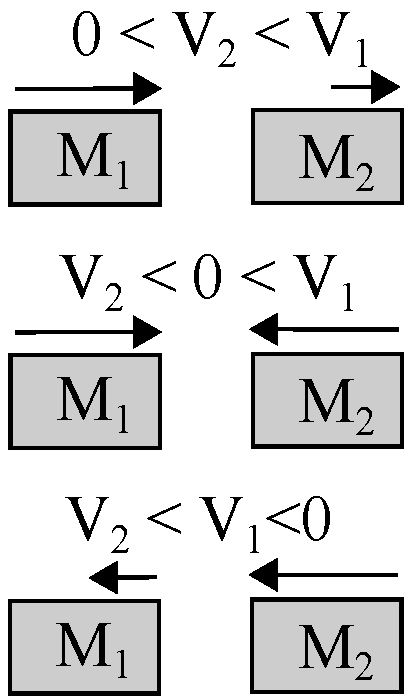
\includegraphics[width=1\linewidth]{Figs/little-momentum0.pdf}
               %\\		\begin{center}(b)\end{center}%\caption{}
              %\label{fig:mom0}
%    \end{subfigure}%
\end{minipage}
\hspace{7mm}
\begin{minipage}{\linewidth/2}
%\qquad
%\begin{subfigure}{0.52\linewidth}
                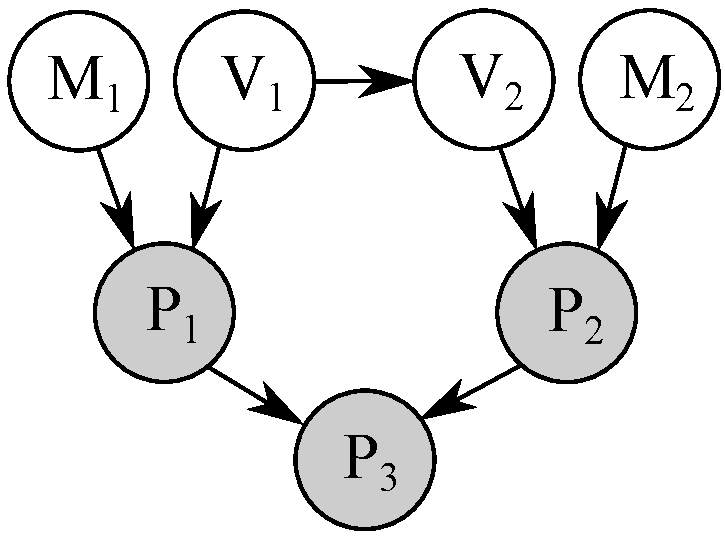
\includegraphics[width=0.80\linewidth]{Figs/little-momentum1.pdf}
                %\\		\begin{center}(b)\end{center}%\caption{}
                %\label{fig:mom00}
    %   \end{subfigure}%
%\end{center}
\end{minipage}
\vspace{3mm}\\
(a) \hspace{25mm}(b)
%\vspace{-1mm}
\caption{\footnotesize 
Collision of masses $M_1$ and $M_2$ with velocities $V_1$ and $V_2$ and momenta $P_1$ and $P_2$. 
(a) Collision happens if and only if $V_1>V_2$. (b) Corresponding Bayesian network. The non-filled and filled Filled circles represent stochastic and deterministic random variables respectively.} 
\label{fig:mom2}
\vspace{-4mm}

\end{center}
\end{figure}

%%%%%%%%%%%%%%%%%%%%%%%%%%%%%%%%%%%%%%%%%%%%%%%%%%%%%%%%%%%%%%%%%%%%%%%%%%

%%%%%%%%%%%%%%%%%%%%%%%%%%%%%%%%%%%%%%%%%%%%%%%%%%%%%%%%%%%%%%%%%%%%%%%%%%
%\vspace{1mm}\\
{\bf Example (Collision). }
\emph{Masses $M_1$ and $M_2$ with velocities $V_1$ and $V_2$ (and consequently momenta $P_1 = M_1 V_1$ and $P_2 = M_2 V_2$) collide to form a single mass ($M_1 + M_2$) with momentum $P_3 = P_1 + P_2$ (assuming that there is no dissipation).
Masses and velocities are unknown but 
their prior distributions are given as follows (note that as Figure~\ref{fig:mom0} shows, a collision only happens if $V_2 < V_1$):  
}%end \emph
\begin{align*}
&\pr(M_1) = \mathcal{U}(0.1, \, 2.1) 
&&\pr(M_2) = \mathcal{U}(0.1, \, 2.1)
\\
&\pr(V_1) = \mathcal{U}(-2, \, 2)
&&\pr(V_2 \, | \, V_1) = \mathcal{U}(-2, \, V_1)
\end{align*} 
\emph{
The conditional dependencies of these random variables are illustrated in 
Figure~\ref{fig:mom00}.
Conditioned on the observation $P_3 = 3$, the posterior joint distribution of $M_1$, $M_2$, $V_1$ and $V_2$ is desired. 
\hspace*{\fill} $\diamond$} %\emph

Despite its humble appearance, the solutions that the existing probabilistic inference tools provide for this model are quite unsatisfactory. 
As a matter of fact, we are unaware of any existing general inference framework that 
handles observed deterministic relationships between random variables!\footnote{
In BUGS \emph{logical nodes} cannot be given data or initial values.
in PyMC deterministic variables have no \emph{observed flag}. 
Stan throws error: ``attempt to assign variable in wrong block'', Anglican//TODO}

Let's take a look on the nature of the problem by manually carrying on the computations required for MCMC sampling:
It can easily be seen that in the Collision example, the prior joint probability of masses and velocities is as follows:

{\footnotesize
\begin{equation}  
\label{e:col-prior}
\pr(M_1, M_2, V_1, V_2)  
=
\begin{cases}
\frac{1}{16 V_1 + 32} &{\text{if }\scriptstyle 0.1<M_1<2.1, \, 0.1<M_2<2.1,}\\
							 &{\;\;\, \scriptstyle -2<V_1<2, \, -2<V_2 < V_1}\\
 \otherwise{0}
 \end{cases}
\end{equation}
}
which is a 4 dimensional function from which samples can be taken fairly easily. 
Since $P_3 = M_1 V_1 + M_2 V_2$, the likelihood of the evidence is a 0-variance conditional distribution:
\begin{equation}
\label{e:col-likelihood}
\pr(P_3 = 3 \,|\, M_1, V_1, M_2, V_2) = \delta[3 - (M_1 V_1 + M_2 V_2)]
\end{equation}
where $\delta[\cdot]$ denotes Dirac delta. 
By Bayes rule, the posterior $\pr(M_1, M_2, V_1, V_2 \,|\, P_3 = 3)$
is proportional to the product of equations (\ref{e:col-prior}) and (\ref{e:col-likelihood}) 
that despite being a 4-dimensional function, its mass is concentrated on a 3 dimensional \emph{hypersurface} {\footnotesize$M_1 V_1 + M_2 V_2 = 3$}. 

In general, observation of an algebraic function of an $N$-dimensional prior often leads to a posterior mass concentrated in an $N-1$-dimensional hyperspace and existence of more deterministic constraints/relationships increases the difference between the dimensionality of the original space and the manifold on which the posterior is concentrated.  
If this dimensionality mismatch is not taken into account, sampling from such posterior distributions via sampling is impossible.\footnote{As a more tangible example, note that taking sample from a curve via random walk in a 3D continuous space is impossible.}  

The solution that the existing MCMC-based frameworks suggest is to approximate the observed deterministic relation by a stochastic relation via adding noise to the observation (measurement error).
For example the r.h.s of equation (\ref{e:col-likelihood}) would be 
approximated with a normal distribution $N(3 - M_1 V_1 - M_2 V_2, \sigma_\eta)$  
where the standard deviation $\sigma_\eta$ is the noise parameter.
Using this trick, it is guaranteed that the posterior is equidimensional with the space of prior (i.e.\ its ambient space) and therefore, sampling from it is possible.
Nonetheless, in practice such a technique does not help much:
If the noise parameter is chosen to be large, even in simple models the samples taken from the approximated posterior may lead to poor simulations of the correct posterior.
If it is chosen to be small, despite the preservation of the dimensionality, the approximated posterior mass would be dense in tinny regions on which the performance of MCMC methods is notoriously unsatisfactory ref(Cooper[5]->Dynamic scaled sampling//todo). The approximation bounds become arbitrary large and mixing rate deteriorates slowly ref(Dynamic scaled sampling)...  
  
%The the deterministic constraint: 
%corresponds to a 0-variance conditional distribution: 
%$$
%\pr(P_3 \,|\, M_1, V_1, M_2, V_2) = \delta[P_3 - (M_1 V_1 + M_2 V_2)] = 3
%$$

.

.

.

Unfortunately, 
beyond the limit of linear relationships, such as $Z = X_1 + X_2$, 
current probabilistic inference systems cannot handle deterministic constraints.
BUGS \cite{lunn2009bugs}, the popular software for analysis of statistical models, 
totally disallows deterministic relationships between continuous random variables.

Families of distributions such as \emph{conditional linear Gaussians (CLG)} \cite{lauritzen2001stable}
allow linear deterministic constraints but as mentioned, inference in the presence of nonlinear deterministic constraints on continuous random variables is still an open problem.

In this paper we solve this problem for a large class of nonlinear multivariate algebraic deterministic constraints in the form of polynomial fractions. 
Our main contributions are:
\begin{itemize}
\item Introducing  an expressive class of functions 
(called PPPFs for \emph{Polynomial-Piecewise Polynomial Fractions}) that facilitates inference in the presence of  linear/nonlinear algebraic deterministic constraints.
\item Presenting an efficient inference method (called \emph{Symbolic Gibbs}) that matches well with the provided model and handles deterministic constraints.  
\end{itemize}

%The proposed class if expressive functions includes 
%Our first contribution is to propose an extremely expressive class of functions for inference in graphical %models (such as Bayesian networks, Markov random fields, etc.).
PPPFs are piecewise polynomial fractions where the variable space is partitioned by polynomial inequalities.
%To show the importance of fractional functions we note that %and nonlinear partitions we note that 
The key insight is that the algebraic constraints preserved PPPF form after collapsing which immediately extends the application of PPPFs to models with sophisticated deterministic algebraic constraints. 
We note that 
even in simple models such as \emph{collision example}, distributions can be piecewise fractional. 
For example:  
\[
\pr(V_2 \,|\, V_1) = \mathcal{U}(-2, V_1)
=
\begin{cases}
  \case{\scriptstyle (V_2 > -2), \, (V_2 < V_1)}{\frac{1}{V_1 + 2}}\\
 \otherwise{0}
 \end{cases}
\]

To show the critical role of nonlinear partitioning conditions in handling the algebraic deterministic constraints, 
let us solve equation~\ref{eq:moment-constraint} for a variable (e.g.\ $V_2$):
$V_2 = \frac{3 - M_1 V_1}{M_2}$) and modify $\pr(V_2 \,|\, V_1)$ by substituting $V_2$ with its the solution.
We will see that this substitution leads to $\pr(V_2 \,|\, V_1, P_3 = 3)$:
\begin{equation}
\label{e:fractional-constraint}
\begin{cases}
  \case{(\frac{3 - M_1 V_1}{M_2} > -2) , \, (\frac{3 - M_1 V_1}{M_2} < V_1)}{\frac{1}{V_1 +2}}\\
  \otherwise{0}
  \end{cases}
\end{equation}
Clearly, this transformation has created a piecewise function with non-linear partitioning conditions.

Recently, piecewise polynomials have attracted attention.
So far, piecewise polynomials with hyperrectangular, hyper-rhombus and linear partitioning constraints have been used in Bayesian networks \cite{shenoy2011inference,shenoy2012two,Sanner:12}.
%hyperrectangular-piecewise polynomials \cite{shenoy2011inference,shenoy2012two,Sanner:12},
%hyper-rhombus-piecewise polynomials \cite{shenoy2012two} and the most general so far, linear-piecewise polynomials \cite{Sanner:12} have been used for inference in Bayesian networks.\footnote{ By \emph{A-piecewise B} we refer to piecewise functions where the function value in each partition is in class \emph{B} and the conditions partitioning the space of variables are (conjunctions of functions) in class \emph{A}.}
These models can only handle linear dependencies and 
our model is more expressive than all of them. 
%This, for the first time, enables probabilistic inference be carried on a large domain of interesting and new  applications.  

The second contribution, as mentioned, is a new variation of Gibbs sampling.  
Gibbs samplers are robust in the sense that they do not need any parameter tuning.
However, they are computationally expensive since to take a single sample they require to compute many univariate integrals (to generate the CDFs of conditional distributions).
We notice that a large subset of PPPFs have closed form (symbolic) integrals. 
The idea of Symbolic Gibbs is to compute a single analytic integral for each variable by keeping the remaining variables uninstantiated. 
The actual process of CDF computation per sample  
simply involves instantiation of the already computed CDFs rather than computing them on the fly.
This dramatically decreases the amount of necessary computations and as our experimental results show, it improves the performance significantly.

In the following sections after a brief introduction to Graphical models, 
followed by an algorithm for inference in the presence of deterministic constraints.
We then explain the restrictions of PPPFs, compare our method with other samplers and conclude. 

\section{Graphical Models (GMs)}
Let $\vec{X} = \{X_1, X_2, \ldots\}$ be a set of random variables with realizations in the form 
$\vec{x} = \{x_1, x_2, \ldots\}$.\footnote{
As a common abuse of notation, in case there is no ambiguity, we do not distinguish between random variables and their realizations; e.g., we abbreviate $\pr(X_i = x_i)$ with $\pr(x_i)$.}
$\vec{X}$ may contain discrete and continuous variables. 
However, for the sake of notational consistency, %and since the problems tackled in this paper only hold for continuous variables, 
we only consider continuous models throughout. 
Note that inference in presence of discrete deterministic constraints is trivial.
Therefore, generalization of the presented framework to hybrid discrete/continuous models is straightforward.   

To cover both directed and undirected graphical models we use
\emph{factor graph} notation \cite{kschischang2001factor}
and represent a joint probability distribution $\pr(\vec{X})$ in a factorized form as follows: 
\begin{equation}
\label{e:factor-graph}
\pr(\vec{X}) = \frac{1}{C} \prod_{\Psi \in \boldsymbol\Psi} \Psi (\vec{X})
\end{equation}
where 
$\Psi(\vec{X})$ is a non-negative, real-valued potential function (of a subset of $\vec{X}$) and $C$ is a (not necessarily known) normalization constant.
%The inference procedure that will be presented does not require the normalization constant be known. 

If the valuation of variables $\bvec{E} \subset \bvec{X}$ is observed,
the joint probability of the remained variables $\bvec{X} \backslash \bvec{E}$ conditioned on the observation ($\bvec{E} = \bvec{e}$) is simply proportional to $\pr(\bvec{X})$ in which $\bvec{E}$ is instantiated by $\bvec{e}$:
\begin{equation}
\label{e:posterior-joint}
\pr(\bvec{X} \backslash \bvec{E} \,|\, \bvec{e}) \propto 
\pr(\bvec{X} \backslash \bvec{E}, \bvec{E} = \bvec{e}) \propto
\prod_{\Psi \in \boldsymbol\Psi} \Psi (\vec{X})|_{\bvec{E} \leftarrow \bvec{e}}
\end{equation}
Provided with (non-normalized) $\pr_{\bvec{e}}(\cdot)$ with dimensionality reduced from $|\bvec{X}|$ to $|\bvec{X}| - |\bvec{E}|$, probabilistic inference is facilitated. 
For example, 
the \emph{posterior} probability of \emph{query} variables $\vec{Q} \subset \vec{X}$ 
%given \emph{evidence} variables $\vec{e} \subset \vec{x}$ 
is computed by marginalizing variables that are not in the query or evidence,
$\{W_1, \ldots, W_k\} := \vec{X} \backslash (\vec{Q} \cup \vec{E})$:
\begin{equation}
\label{e:inference}
\pr(\vec{Q} \,|\, \vec{e}) \propto 
\int_{w_1 = -\infty}^{\infty} \!\!\!\!\!\! \cdots \int_{w_k = -\infty}^{\infty}
%\prod_{\Psi \in \boldsymbol\Psi} \Psi(\vec{x})
\!\!\!\!\!\!\!\! \pr_{\bvec{e}}(\bvec{Q}, w_1, \ldots, w_k )
\, d_{w_1} \ldots d_{w_k}
\end{equation}
%We will shortly show that unlike the conventional graphical models, in models with deterministic constraints, the creation of joint distribution of unobserved variables requires more computations. We first formalize such models. 
\subsection{Inference in GMs}
\textbf{Closed form inference.}
The main challenge for closed inference is the computation of multiple integrals required for marginalization (equation~\ref{e:inference}).
There are a few classes of functions which are closed under integration.
However, none of these classes can handle deterministic constraints beyond the level of linear constraints.
\\
\textbf{Monte Carlo methods}
%An alternative to exact inference is to approximate the joint distribution by a set of samples drawn from it using Monte Carlo methods. By the law of large numbers, this approximation is asymptotically unbiased. Using samples, the costly marginalization operation is avoided since the conditional probability $\pr(\bvec{q} \,| \, \bvec{e})$ is simply approximated by the number of samples satisfying $\bvec{q} \cap \bvec{e}$ divided by the number of samples satisfying $\bvec{e}$.
%Note that unlike other approximate methods, inference via sampling leads to asymptotically unbiased solutions i.e.\ by taking sufficient number of samples, the \emph{posterior} can be approximated by an arbitrary precision.
Approximating the posterior distribution via drawing samples from it by Monte Carlo methods 
provides an asymptotically unbiased tool that completely avoids the hassle of multiple integrations required in closed-form sampling.   
Three major such methods are as follows:

\emph{Rejection sampling}: In this method, to draw a sample from 
a distribution $p(\bvec{X})$, a sample $\bvec{x}$ is taken from another distribution $q(\bvec{X})$
such that $p(\bvec{X})/q(\bvec{X})$ is bound by a known constant $c$
and samples can be taken from $q(\bvec{X})$ efficiently.
The produced sample is accepted with probability $p(\bvec{x}) / c q(\bvec{x})$, 
otherwise it is rejected and the process is repeated. 

\emph{Metropolis-Hastings (MH)}:
To draw a new sample $\bvec{x}^{(t)}$ from a distribution $p(\bvec{X})$, given a previously taken sample $\bvec{x}^{(t-1)}$, 
MH takes a sample $\bvec{x}'$ from a symmetric \emph{proposal density} $q(\bvec{X} |\, \bvec{x}^{(t-1)})$. 
%from which samples can be taken efficiently 
%(often an isotropic \emph{Gaussian} centered at $\bvec{x}^{(t-1)}$). 
With probability $\min \big(1, p(\bvec{x}')/p(\bvec{x}^{(t-1)}) \big)$, 
$\bvec{x}'$ is accepted as the next sample ($\bvec{x}^{(t)} \leftarrow \bvec{x}'$), otherwise, $\bvec{x}^{(t)} \leftarrow \bvec{x}^{(t-1)}$. 
Choosing a good \emph{proposal} is problem-dependent and requires tuning. 


\emph{Gibbs sampling}:
Gibbs is a robust sampling tool in the sense that it does not require known bounds, tuned proposal densities or parameters.
Drawing a sample for $\bvec{X} = (X_1, \ldots, X_N)$ takes place in $N$ steps.
In the $i$-th step, $X_i$ is sampled conditioned on the last realization of the others:
$x_i \sim \pr(X_i \,|\, \bvec{x}_{-i})$. 
To perform this task, the following univariate \emph{Cumulative Distribution Function} (CDF)
is computed by equation~(\ref{e:cdf}) and samples are taken by inverse transform sampling. 
{\footnotesize
\begin{equation}
\label{e:cdf}
F(X_i  \,|\, \bvec{x}_{-i}) 
\propto
\int_{-\infty}^{X_i} \!\!\!\! \pr(X_i = t, \bvec{x}_{-i}) \, d  t
\end{equation} 
}
%Computation of $N$ univariate integrals per sample is costly and this makes Gibbs sampling a relatively slow sampler. However, we will show that the family of PPPF functions, the performance of Gibbs sampling can be improved significantly.

In the next section, we formalize GMs with deterministic variables. 

%%%%%%%%%
\section{Graphical Models with Linear/Non-linear Deterministic Constraints}
Consider a graphical model with random variables $\bvec{X} := \bvec{Y} \cup \bvec{Z}$
where $\bvec{Y}$ and $\bvec{Z}$ are respectively called \emph{stochastic} and \emph{deterministic}  sets of random variable.

In the network specification that we are concerned with, 
for each deterministic random variable $Z \in \bvec{Z}$ there exists exactly one \emph{associated potential function} 
$\Psi_Z := \delta[Z - G^Z]$ (indicating the deterministic dependency $Z = G^Z$)
where $\delta[\cdot]$ is \emph{Dirac delta} function and $G^Z$, the \emph{logical value} of $Z$,  is an expression that does not involve $Z$ (i.e.\ $Z \not\in \textsc{Scope}(G^{Z})$).\footnote{
As an instance, in the \emph{collision example}, $G^{P_1} = M_1 V_1$.
}


We say $Z\in \bvec{Z}$ is a \emph{deterministic parent} of $Z' \in \bvec{Z}$ if 
$Z \in \textsc{Scope}(G^{Z'})$. 
The dependency of deterministic random variables to each other should form a \emph{directed acyclic graph} (DAG). That is, a deterministic random variable cannot be a parent (or an ancestor) of its deterministic parents. This restriction guarantees that the deterministic variables are not defined recursively.
%\begin{equation*}
%\forall Z, Z' \in \bvec{Z} \qquad Z \in \textsc{Scope}(G^{Z'}) \Rightarrow Z' \not\in \textsc{Scope}(G^Z)
%\end{equation*}
$\boldsymbol{\Psi^D} :=\{\Psi_Z \,|\, Z \in \bvec{Z}\}$ is the set of deterministic potentials.

We assume the remained potentials 
$\boldsymbol{\Psi} \backslash \boldsymbol{\Psi^D}$ 
are non-negative function that do not involve Dirac deltas. We refer to such factors as \emph{stochastic potentials}.
We impose no restriction on the stochastic potential functions except the obvious requirement that the product of all potentials should be proportional to the joint distribution of all random variables. 
%$q(\bvec{Y}) \propto \pr(\bvec{Y})$.
For the sake of notational simplicity, throughout we assume that the models are converted to a \emph{standard} form with the following characteristics:
\begin{enumerate}
\item The logical values of deterministic random variable only contains stochastic random variables:
\begin{equation}
\label{e:as1}
\forall Z \in \bvec{Z} \qquad \textsc{Scope}(G^Z) \subset \bvec{Y}
\end{equation} 
\item The only stochastic potential in the model is $\Phi$ and $\textsc{Scope}(\Phi) \subset \bvec{Y}$.\footnote{
Therefore, the set of all potentials $\boldsymbol{\Psi} := \boldsymbol{\Psi^D} \cup \{\Phi\}$. %\boldsymbol{\Psi^S}$
} This means that $\Phi \propto \pr(\bvec{Y})$.
\end{enumerate}

%where $\boldsymbol{\Psi^D} :=\{\Psi_Z \,|\, Z \in \bvec{Z}\}$ is the set of deterministic potentials.%and $\boldsymbol{\Psi^S}$ is the set of stochastic (i.e.\ conventional) potentials. 


To covert a network to this form it suffices to: 
 \begin{itemize}
\item In all potentials, substitute (other) deterministic random variables $Z$ with their logical values $G^Z$. 
\begin{equation*}
\forall Z \in \bvec{Z}, \Psi \in \boldsymbol{\Psi}\backslash \{\Psi_Z\} \qquad \Psi \leftarrow \Psi|_{Z \leftarrow G^Z}
\end{equation*}
Pre-order traversal of the DAG dependency structure of $\bvec{Z}$ guarantees that this process satisfies (\ref{e:as1}).  
\item Compute $\Phi$ as the product of all stochastic factors.
\end{itemize} %\footnote{ Nonetheless, note that is practice, in order to carry on symbolic operations such as substitution, simplification and factorization (that will be used shortly), it is often better to multiply the stochastic potentials in later stages of the inference. 
%}

For example, a standard form for the Collision model is:
$\Phi := \pr(M_1, M_2, V_1, V_2)$ (as in equation (\ref{e:col-prior})),
and $\boldsymbol{\Psi^D} := \{\Psi_{P_1}, \Psi_{P_2}, \Psi_{P_3}\}$ 
where $\Psi_{P_1} := \delta[P_1 - M_1 V_1]$,
$\Psi_{P_2} := \delta[P_2 - M_2 V_2]$ and
$\Psi_{P_3} := \delta[P_3 - M_1 V_1 - M_2 V_2]$.



In the next sections, inference in models with \emph{standard} forms is studied.
%%%%%%%%%%%%%%%%%%%%%%%%%%%%%%%%%%%%%%%%%%%%%%%%%%%%%%%%%%%%%%%%%
\begin{comment}
\begin{algorithm}[tb]%[hb!]
\caption{{\sc PosteriorJoint}  
\label{alg:posterior-joint}}
\begin{algorithmic}
%{\small
\STATE {\bf Input: }{
$\mathbb{E} = \{\tuple{E_i, e_i}\}_i$ 
// \emph{\small evidence}\\
%$\bvec{Z} = \{Z\}$, deterministic variables\\
\qquad $\boldsymbol{\Psi} = \boldsymbol{\Psi^D} \cup \boldsymbol{\Psi^S}$ 
 //\emph{set of potentials.
 } }
\STATE {\bf Output} {posterior joint distribution of a subset of variables from which, all other variables can be decided.}

 \vspace{1mm}
%{
%{\bf Begin}//{

\STATE //\emph{{\bf \sc Step 1.} Instantiation of the observed variables:}
	
\FOR{{\bf all} $\tuple{E, e} \in \mathbb{E}$}
\STATE \textbf{for all } $\Psi \in \boldsymbol{\Psi}$ \textbf{ do } $\Psi \leftarrow \Psi|_{E \leftarrow e}$	
\ENDFOR %\textbf{end for}\\

\vspace{1mm}
	
//\emph{{\bf \sc Step 2.} Isolating deterministic variables:}
\FOR{{\bf all} $\Psi_Z = \delta [Z - G^Z] \in \boldsymbol{\Psi^D}$}
	\STATE \textbf{forall }{$\Psi \in \boldsymbol{\Psi}$} \textbf{ do } 
		{$\Psi \leftarrow \Psi|_{Z \leftarrow G^Z}$	}
\ENDFOR
	
 \vspace{1mm}
	
\STATE //\emph{{\bf \sc Step 3.} Joint factor formation:}

\STATE $\pr_{\bvec{e}} \leftarrow \prod_{\Psi \in \boldsymbol{\Psi^S}} \Psi$\\
     %$J \leftarrow 1$\\
	%\ForAll{$\Psi \in {\boldsymbol\Psi}^{S}$}
	%{
	%	$J \leftarrow J \otimes \Psi$
	%}
	%\textbf{end for}\\
 \vspace{1mm}
	
\STATE //\emph{{\bf \sc Step 4.} Collapsing determinism:}

\FOR {{\bf all} $\tuple{E, e} \in \mathbb{E}$ \textbf{such that} 
		$E \in \bvec{Z}$}
	\STATE \textbf{let} $\tuple{Y, G^Y} = \textsc{solve}(G^E=e)$ //  \emph{assuming that a unique solution exists.}

\STATE $\pr_{\bvec{e}} \leftarrow \pr_{\bvec{e}}|_{Y \leftarrow G^Y}$ 
	// \emph{substituting $Y$ with its solution}\\	

\ENDFOR
%	\textbf{end for}\\
\STATE {\bf Return} $\pr_{\bvec{e}}$
%}
%}%end small
%}
\end{algorithmic}
\end{algorithm}
%\decmargin{0.5em}
\end{comment}
%%%%%%%%%%%%%%%%%%%%%%%%%%%%%%%%%%%%%%%%%%%%%%%%%%%%%%%%%%%%%%%%%

\section{Inference in GMs with Deterministic (Non)Linear Constraints}
We allow both stochastic and deterministic variables to be observed by evidence.  
We are interested in deterministic variables with associated logical values  
created by elementary arithmetic operators ($+$, $-$, $\times$, $\div$) and therefore 
are in the form of fractions of polynomials.

As mensioned, observed deterministic random variables lead to posterior distributions concentrated on submanifolds of the stochastic variable space.
In Section~\ref{sect:infer1}, we provide an algorithm to restate the posterior distribution of a subset of stochastic random variables in 
a space that matches it in term of dimensionality.

In Section~\ref{???} we 
%This Guaranteeing that the dimensionality of the posterior and its enveloping manifold match,  asymptotically unbiased inference can be performed using MCMC methods.

 
%In order to conduct inference we first compute the posterior joint distribution  (as in equation~\ref{e:posterior-joint}). of non-observed variables. 
%To perform this task, we propose \emph{collapsing} (i.e.\ marginalizing over) all observed and non-observed deterministic variables. The details are presented in the next subsection. 
%Provided with the posterior, the main task of inference is carried out by equation~(\ref{e:inference}). For this task we will rely on Symbolic Gibbs sampling.

{\color{red} .then MODEL ... then Gibbs sampling(?)\\TODO..}

\subsection{Posteriors in GMs with Deterministic Constraints}
\label{sect:infer1}

The aim of this section is to find a posterior joint distribution over a subset $\bvec{X}'$ of stochastic random variables $\bvec{X}$
such that any other variable (either stochastic or deterministic)
can be expressed as a function of $\bvec{X}'$.
The procedure
%, as formalized in Algorithm~\ref{alg:posterior-joint}, 
is as follows: 
\begin{enumerate}
\item \emph{Instantiation of observed variables.} 
In all potentials, observed stochastic and deterministic random variables are instantiated (as in equation~\ref{e:posterior-joint})
\begin{equation*}
\forall \Psi \in \boldsymbol{\Psi} \qquad \Psi \leftarrow \Psi|_{\bvec{E} \leftarrow \bvec{e}}
\end{equation*} 

%
%\item \emph{Isolating deterministic variables.} In all potentials, all deterministic variables $Z$, are 
%substituted with their associated logical value $G^Z$ (so, the potential $\delta[x - G^x]$ itself is replaced by 1). Note that by the definition of Dirac $\delta$, this simply means all deterministic variables are marginalized.
%
%\item \emph{Joint factor formation.} the product of the remaining potentials is computed (as in equation~\ref{e:posterior-joint}).   
%
\item \emph{Dimension reduction} %collapsing determinism 
%What remains is to condition on the deterministic constraints.
For each observed deterministic random variable $Z = c$ (where $c$ is a constant),
$(G^Z - c)$ is solved w.r.t.\ some variable $Y \in \textsc{Scope}(G^Z)$ (assuming that it is solvable %with a single solution 
w.r.t.\ at least one variable).
Let $\textsc{Solve}(G^Z - c; \, Y) := \{y^{1}, y^{2}, \ldots\}$ be the set of such solutions.
$\Phi$ is replaced by:
\begin{equation}
\label{e:core}
\sum_{y^{i} \in \textsc{Solve}(G^Z - c;\, Y)}
\frac{\Phi|_{Y \leftarrow y^{i}}}{
\big|(\partial G^Z / \partial Y) |_{Y \leftarrow y^{i}}
\big|
}
\end{equation}
\end{enumerate}
In the latter phase, Theorem~\ref{theorem1} is utilized consecutively.  
The end result $\Phi$ is proportional to 
$\pr(\bvec{Y}\backslash \bar{\bvec{Y}} \,|\, \bvec{E} = \bvec{e})$ in which 
$\bar{\bvec{Y}}$ is the set of stochastic variables eliminated in the \emph{dimension reduction phase}. 

For instance in the Collision model with evidence ($P_3 = 3$),
In Step 1, $\Psi_{P_3}$ is converted to $\delta[3 - M_1 V_1 - M_2 V_2]$ while the other potentials are not modified.

 In step 2, $(3 - M_1 V_1 - M_2 V_2)$ is solved w.r.t.\ $M_1$\footnote{It could alternatively be solved w.r.t. $V_1$, $M_2$ and $V_2$.}:
\\
$\textsc{Solve}(3 - M_1 V_1 - M_2 V_2; M_1) = \{\frac{3 - M_2 V_2}{V_1}\}$ 
and $\left| \frac{\partial (3 - M_1 V_1 - M_2 V_2)}{\partial M_1} \right| = |V_1|$.
Finally using formulas (\ref{e:col-prior}) and (\ref{e:core}), 
$\pr(M_2, V_1, V_2 \,|\, P_3 = 3)$ is proportional to:
%%
{\footnotesize
\begin{equation}  
\label{e:col-prior2}
%\pr(M_2, V_1, V_2)  =
\begin{cases}
\frac{1}{V_1(16 V_1 + 32)} &{\text{if }\scriptstyle 0<V_1, \, 0.1<\frac{3-M_2 V_2}{V_1}<2.1, \, 0.1<M_2<2.1,}\\
							 &{\;\;\, \scriptstyle -2<V_1<2, \, -2<V_2 < V_1}\\
\frac{-1}{V_1(16 V_1 + 32)} &{\text{if }\scriptstyle V_1<0, \, 0.1<\frac{3-M_2 V_2}{V_1}<2.1, \, 0.1<M_2<2.1,}\\
							 &{\;\;\, \scriptstyle -2<V_1<2, \, -2<V_2 < V_1}\\
 \otherwise{0}
 \end{cases}
\end{equation}
}


\begin{theorem} 
\label{theorem1}
Let {\footnotesize $\pr(Z\!=\!z | x_1, \ldots, x_n) = \delta[f(x_1, \ldots, x_n)-z]$}.
If {\footnotesize$\textsc{Solve}\big( f(x_1, \ldots, x_n) - z ; \, x_1 \big)$} denotes the set of solutions of 
$f(x_1, \ldots, x_n)-z$ w.r.t.\ $x_1$:
\begin{multline}
\label{e:theorem1}
p_{\boldsymbol{X}\backslash X_1 | Z}(x_2, \ldots, x_n \,|\, Z=z) \propto \\
\sum_{x_1^i \in \textsc{Solve}\big( f(\cdot) - z ; \, x_1 \big)} 
\frac{p(X_1=x_1^i, x_2, \ldots, x_n)}
{\Big|\big(\partial f(x_1, \ldots, x_n) / \partial x_1 \big)|_{x_1 \leftarrow x_1^i} \Big|}
\end{multline}
\end{theorem}
\begin{proof}
$p(x_2, \ldots, x_n \,|\, Z=z)$ is proportional to
\begin{align}
%p(x_2, \ldots, x_n \,|\, Z=z) = \\
%
%\int_{x_1=-\infty}^{\infty}p(x_1, \ldots, x_n \,|\, Z=z) dx_1 \propto \\
%
%&\int_{x_1=-\infty}^{\infty}p(x_1, \ldots, x_n, Z=z) dx_1 =\\
%
&\int_{x_1=-\infty}^{\infty}p(x_1, \ldots, x_n)p(Z=z \,|\, x_1, \ldots, x_n) dx_1 \notag\\
%
=&\int_{x_1=-\infty}^{\infty}p(x_1, \ldots, x_n)
\delta[f(x_1, \ldots, x_n) - z] dx_1 
\label{e:fand}
\end{align}
According to \cite{gel1964generalized}
there is a unique way to define the composition of Dirac delta with 
arbitrary functions $h(x)$:
\begin{equation}
\label{e:gelfand}
\delta(h(x)) = \sum_{i} \frac{\delta[x - r_i]}{|\partial h(x)/\partial x|}
\end{equation}
where $r_i$ are all (real and simple) roots of $h(x)$ and $h(x)$ is continuous and differentiable in the the root points. By (\ref{e:gelfand}), (\ref{e:fand}) and 
\emph{Tonelli's theorem}\footnote{Tonelli's theorem says that for non-negative functions, sum and integral are interchangeable.} 
$\pr(x_2, \ldots, x_n \,|\, Z = z) \propto$
\begin{equation*}
\sum_{x_1^i \in \textsc{Solve}\big( f(\cdot) - z ; \, x_1 \big)} \!\!\!\!\!\!\!\!
\frac{\int_{x_1 = -\infty}^{\infty} p(x_1, x_2, \ldots, x_n)  \delta[x_1 - x_1^i] d x_1}
{\Big|\big(\partial f(x_1, \ldots, x_n) / \partial x_1 \big)|_{x_1 \leftarrow x_1^i} \Big|}
\end{equation*}
which implies (\ref{e:theorem1}).
\end{proof}

Theorem~\ref{theorem1} can alternatively be proved via transformation of variables 
(to derive $\pr(z, x_2, \ldots. x_n)$ from $\pr(x_1, \ldots, x_n)$) and utilizing \emph{Inverse function theorem}.

A subtle point in conditioning on determinism is that apparently equivalent deterministic observations may lead to different posteriors. For example evidence $(E_1 = 0)$ where $\pr(E_1)= \delta[E_1 - M V + 3]$ and 
evidence $(E_2 = 0)$ where $\pr(E_2) = \delta[E_2 - M + \frac{3}{V}]$ lead to different posteriors. 
The reason can be understood by considering Dirac deltas as the limit of normal distributions with $\sigma \rightarrow 0$.
(Note that 
$\mathcal{N}(x - MV + 3, \sigma) \neq \mathcal{N}(x -M + \frac{3}{V}, \sigma)$).
Therefore, the canonical way to express a deterministic relationship is a form to which one would add noise if one had to approximate the determinism which is model-dependent. 
  

%A subtle point in conditioning on deterministic relationships is that the resulting density is affected by the value of the prior in the limit of the ambient space surrounding the posterior hypersurface (or submanifold). Therefore, an observed deterministic relationship  (e.g.\ $M_1 V_1 = 3$) cannot be represented by equivalent forms (e.g.\ $M_1 - \frac{3}{V_1} = 0$) in the same way the noisy estimation of the former and latter produce different distribution (e.g.\ $N((M_1 V_1 - 3), \sigma)$ differs $N((M_1 - \frac{3}{V_1}), \sigma)$).


\subsection{Symbolic Gibbs Sampling}
++++++

%The output of this algorithm is a non normalized joint distribution of  a subset of none-deterministic variables. Provided with this joint, the marginal distribution of all query variables (either probabilistic or deterministic) can be computed by means of sampling as will be discussed later.

%Note that these operations alter the normalization constant and the resulting function is only proportional to the corresponding joint distribution. However, most inference algorithms do not require normalization.Some of these algorithms are provided in the next section. However, prior to that we discuss the limitations of Algorithm~\ref{alg:posterior-joint} 
The family of deterministic constraints studied in this work includes polynomial fractions.
For this family, 
the unique solution assumption (required in Step 4 of Algorithm~\ref{alg:posterior-joint})
in general holds if $G^Z$, the logical values of deterministic variables, are linear w.r.t. some variables.
That is, for some variable $Y$, $G^Z$ can be stated as: 
{\footnotesize
\begin{equation}
\label{eq:evidence-form}
G^Z = \frac{\mathcal{A} \cdot Y + \mathcal{B}}{\mathcal{C} \cdot Y + \mathcal{D}}
\end{equation}
}
where $\mathcal{A}$ to $\mathcal{D}$ are constant or univariate/multivariate polynomials and $Y$ is not in their scopes.

+++++

Our symbolic Gibbs sampling is based on a simple but significantly useful insight.
Namely, if the multivariate function $\pr(X_1, \ldots, X_N)$
has an analytic (symbolic) integral for all its variables $X_i$,
then, instead of using equation~\ref{e:cdf}, we map each variable $X_i$ to its corresponding symbolic CDF: 
{\footnotesize
\begin{equation}
\label{e:cdf-symbolic}
F(X_i  \,|\, \bvec{X}_{-i}) 
\propto
\int_{-\infty}^{X_i} \!\!\!\!\! \pr(X_i = t , \bvec{X}_{-i}) \, d  t
\end{equation} 
}
Note that the difference between (\ref{e:cdf}) and (\ref{e:cdf-symbolic}) is that in the former, 
all variables except $X_i$ are already instantiated therefore 
$F(X_i  \,|\, \bvec{x}_{-i})$ is a univariate function but in  (\ref{e:cdf-symbolic}), 
although variables $\bvec{X}_{-i}$ are treated as constants but they are kept uninstantiated and symbolic.
As a result, $F(X_i \,|\, \bvec{X}_{-i})$ is a multivariate analytic function. 
%as Algorithm~\ref{alg:analytic-cdf} shows, 
%we can create a map from variables $X_i$ to their corresponding closed-form CDFs.

The map (called {\sc VarToCDF}) from variables $X_i$ to their symbolic CDFs
$F(X_i \,|\, \bvec{X}_{-i})$ is passed to the main symbolic Gibbs sampling procedure in Algorithm~\ref{alg:symbolic-gibbs}.
During the sampling process, 
to sample $x_i \sim \pr(X_i \,|\, \bvec{x}_{-i})$
it is sufficient to get the (multivariate) symbolic CDF associated to $X_i$ from the map
and instantiate it with $\bvec{x}_{-i}$ to obtain the appropriate univariate CDF.

By this method, instead of computing $N \times T$ integrals for $T$ samples, only $N$ integrals are computed and 
$N \times T$ function instantiations are performed. But function instantiation is much faster than integration.
Therefore, the algorithm leads to a major improvement in speed.

What remains is to show that a large subset of PPPF functions indeed have closed-form integrals. 

%%%%%%%%%%%%%%%%%%%%%%%%%%%%%%%%%%%%%%%%%%%%%%%%%%%%%%%%%%%%%%%%%

\begin{algorithm}[hb!]%[tb]
\caption{{\sc SymbolicGibbs}  
\label{alg:symbolic-gibbs}}
\begin{algorithmic}
 \STATE {\bfseries Input:}
{$\bvec{X} := \tuple{X_1, \ldots, X_N}$, 				\hspace*{\fill}// \emph{\small random variables} \\
 $\bvec{x}^{(0)} := \tuple{x_1^{(0)}, \ldots, x_N^{(0)}}$, 	\hspace*{\fill}// \emph{\small initial values} \\
{\sc VarToCDF}, 								\hspace*{\fill}//\emph{\small variables to analytic CDFs map} \\
 $T$ 										\hspace*{\fill}// \emph{\small number of desired samples } }
\STATE{\bf Output:}{ list of taken samples}
//%\BlankLine
{\small
%{\bf Begin}//  
\FOR{$t= 1, 2, \ldots T$}
	 \STATE $\tuple{x_1^{(t)}, \ldots, x_N^{(t)}} \leftarrow \tuple{x_1^{(t-1)}, \ldots, x_N^{(t-1)}}$    
	\FOR{ {\bf each} $X_i \in \bvec{X}$}
		\STATE $F(\bvec{X}) \leftarrow \textsc{VarToCDF}.\text{get}(X_i)$ //\emph{analytic CDF w.r.t.\ $X_i$:}
		\STATE //\emph{univariate CDF w.r.t.\ $X_i$:}
		\STATE 	$G(X_i) \leftarrow F(x_1^{(t)}, \ldots, x_{i-1}^{(t)}, X_i, x_{i+1}^{(t)}, \ldots, x_N^{(t)})$ 
		\STATE //\emph{$G(\infty)$ is the normalization constant}
		\STATE $x_i^{(t)} \leftarrow \textsc{InverseTransformSample}(\frac{G(X_i)}{G(\infty)})$
	\ENDFOR %end for each x_i
\ENDFOR %end for t
\STATE {\bf Return} {$\big\langle
			\tuple{x_1^{(1)}, \ldots, x_N^{(1)}}, \ldots, 
			\tuple{x_1^{(T)}, \ldots, x_N^{(T)}}
		\big\rangle$}\;
%	ForEach{}{
%	
%	}
%	\textbf{end for}\\
 %  }
   %\textbf{end for}\\   
%}
} %end small
\end{algorithmic}
\end{algorithm}

%%%%%%%%%%%%%%%%%%%%%%%%%%%%%%%%%%%%%%%%%%%%%%%%%%%%%%%%%%%%%%%%%
%..........................
\begin{figure*}
\begin{center}
%\vspace{-1mm}
\begin{minipage}[b]{\nn\textwidth}
                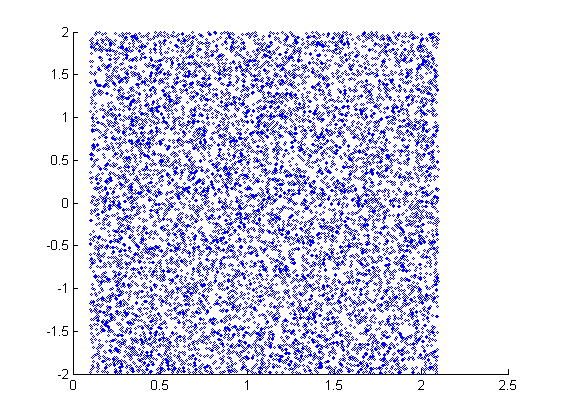
\includegraphics[width=1\textwidth]{Figs/col_m1_v1.png}
                %\caption{}
                %\label{fig:mom1}
        \end{minipage}%
%
%\hspace{20mm}
\begin{minipage}[b]{\nn\textwidth}
                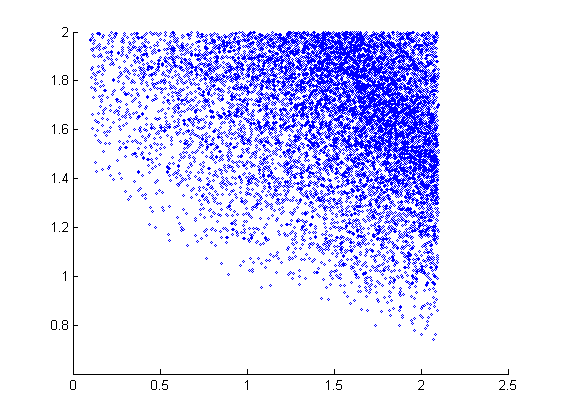
\includegraphics[width=1\textwidth]{Figs/col_m1v1_p3.png}
                %\caption{}
                %\label{fig:mom2}
        \end{minipage}%
\begin{minipage}[b]{\nn\textwidth}
                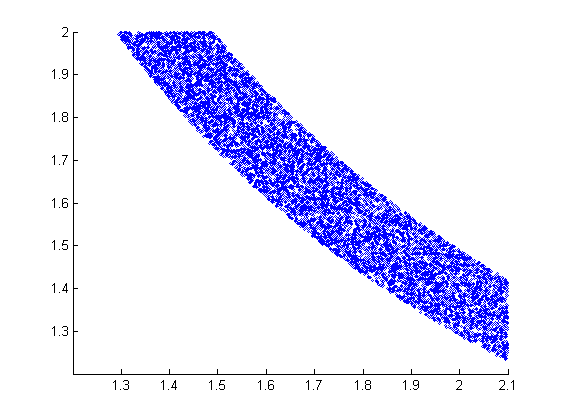
\includegraphics[width=1\textwidth]{Figs/col_m1v1_when_p_is_3_and_v2_is_0_dot_2.png}
                %\caption{}
                %\label{fig:mom2}
        \end{minipage}%
\hspace{4mm}
%\\
\begin{minipage}[b]{\nn\textwidth}
                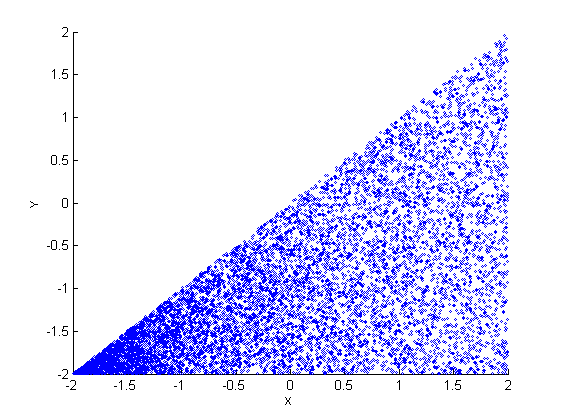
\includegraphics[width=1\textwidth]{Figs/col_v1v2.png}
                %\caption{}
                %\label{fig:mom2}
        \end{minipage}%
\begin{minipage}[b]{\nn\textwidth}
                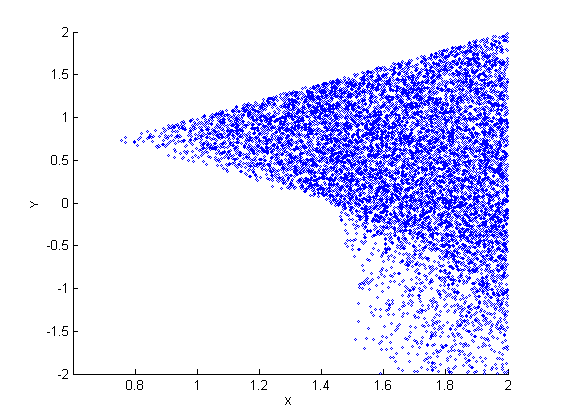
\includegraphics[width=1\textwidth]{Figs/col_v1v2whenPis3.png}
                %\caption{}
                %\label{fig:mom2}
        \end{minipage}%
\begin{minipage}[b]{\nn\textwidth}
                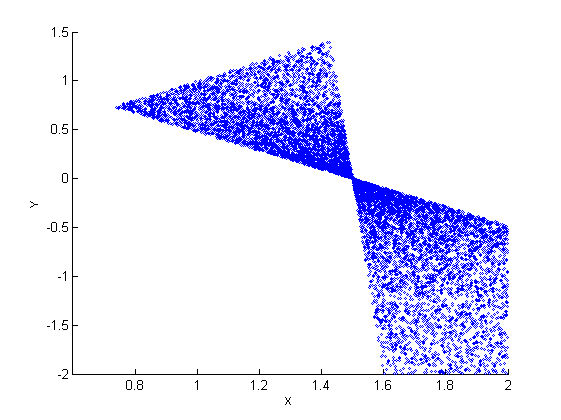
\includegraphics[width=1\textwidth]{Figs/colV1V2givenPis3M1is2.png}
                %\caption{}
                %\label{fig:mom2}
        \end{minipage}%
\end{center}
\vspace{-1mm}
\caption{\footnotesize
prior/posterior joint distributions of pairs of random variables in the \emph{collision} example. 
(a) $\pr(M_1, V_1)$,
(b) $\pr(M_1, V_1 \, | \, P_3 = 3)$,
(c) $\pr(M_1, V_1 \, | \, P_3 = 3, V_2 = 0.2)$,
(d) $\pr(V_1, V_2)$,
(e) $\pr(V_1, V_2 \, | \, P_3 = 3)$,
(f) $\pr(V_1, V_2 \, | \, M_1 =2, P_3 = 3)$
} 
\label{fig:mom}
%\vspace{-4mm}
\end{figure*}
%%%%%%%%%%%%%%%%%%%%%%%%%%%%%%%%%%%%%%%%%%%
\begin{figure*}
\begin{center}
%\vspace{-1mm}
\begin{minipage}[b]{\nn\textwidth}
                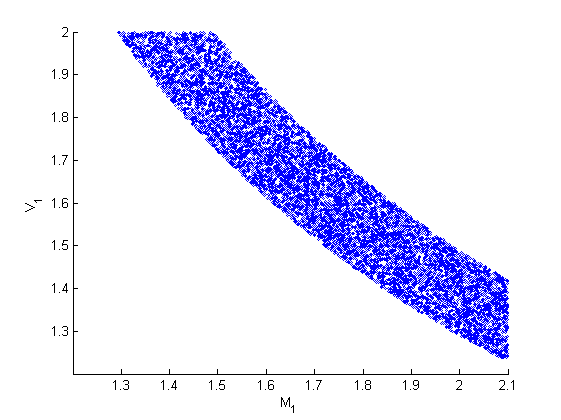
\includegraphics[width=1\textwidth]{Figs2/col_c_rej10000.png}
                %\caption{}
                %\label{fig:mom2}
        \end{minipage}%
\begin{minipage}[b]{\nn\textwidth}
                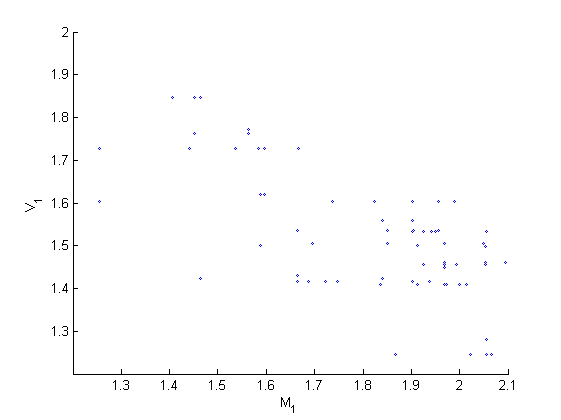
\includegraphics[width=1\textwidth]{Figs2/col_m1v1_p3v2_anglican1000.png}
                %\caption{}
                %\label{fig:mom1}
        \end{minipage}%
%
%\hspace{20mm}
\begin{minipage}[b]{\nn\textwidth}
                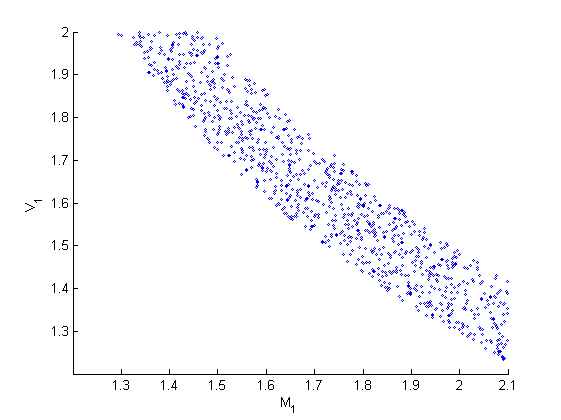
\includegraphics[width=1\textwidth]{Figs2/col_c_rej1000.png}
                %\caption{}
                %\label{fig:mom2}
        \end{minipage}%
\begin{minipage}[b]{\nn\textwidth}
                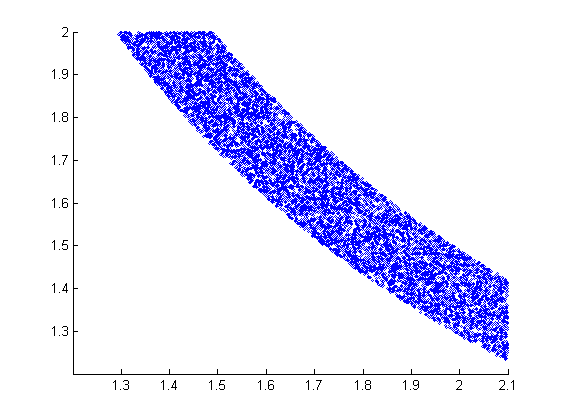
\includegraphics[width=1\textwidth]{Figs/col_m1v1_when_p_is_3_and_v2_is_0_dot_2.png}
                %\caption{}
                %\label{fig:mom2}
        \end{minipage}%
%\hspace{4mm}
%\\
\begin{minipage}[b]{\nn\textwidth}
                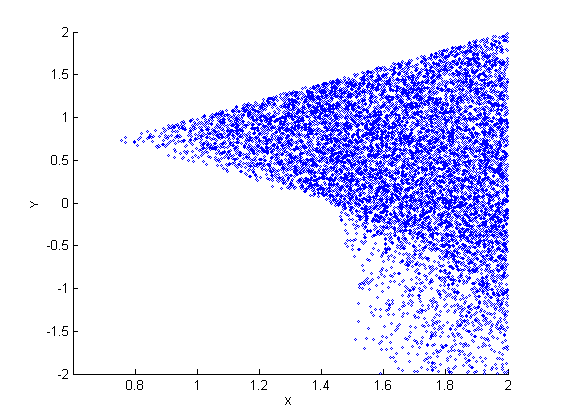
\includegraphics[width=1\textwidth]{Figs/col_v1v2whenPis3.png}
                %\caption{}
                %\label{fig:mom2}
        \end{minipage}%
\begin{minipage}[b]{\nn\textwidth}
                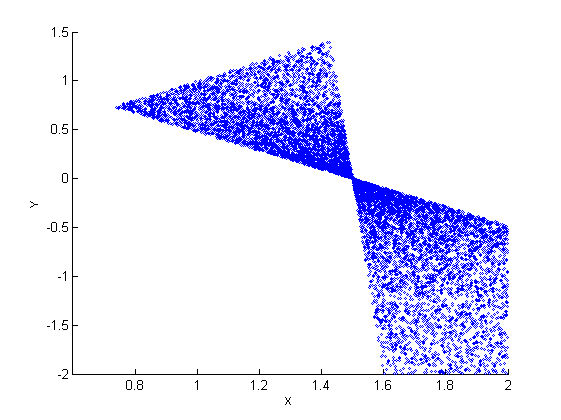
\includegraphics[width=1\textwidth]{Figs/colV1V2givenPis3M1is2.png}
                %\caption{}
                %\label{fig:mom2}
        \end{minipage}%
\end{center}
\vspace{-1mm}
\caption{\footnotesize
prior/posterior joint distributions of pairs of random variables in the \emph{collision} example. 
(a) $\pr(M_1, V_1)$,
(b) $\pr(M_1, V_1 \, | \, P_3 = 3)$,
(c) $\pr(M_1, V_1 \, | \, P_3 = 3, V_2 = 0.2)$,
(d) $\pr(V_1, V_2)$,
(e) $\pr(V_1, V_2 \, | \, P_3 = 3)$,
(f) $\pr(V_1, V_2 \, | \, M_1 =2, P_3 = 3)$
} 
\label{fig:mom}
%\vspace{-4mm}
\end{figure*}

\section{Piecewise Algebraic Graphical Models}
In this section, we put things together and provide our complete model.
The requirements for the class of potential functions (factor forms) are as follows:
\begin{itemize}
\item Factor forms should be as expressive as possible to be able simulate different density forms.  
\item Factor forms should be closed under multiplication and polynomial fractional substitutions such as 
the r.h.s.\ of equation~(\ref{eq:evidence-form}). Otherwise, \emph{joint factor formation} and multiple substitutions in the \emph{collapsing determinism} phase of 
Algorithm~\ref{alg:posterior-joint} can be problematic.
\item A single analytical integration 
(i.e.\ integrating w.r.t.\ a single variable while keeping the rest of variables symbolic) should produce a closed-form structure (the requirement of Symbolic Gibbs).
\end{itemize}   

Our proposition is the use of 
the class of \emph{Polynomial-Piecewise Polynomial Fractions} (PPPFs); That is,   
functions in the form:

\begin{equation}
\label{e:ppf}
f = 
  \begin{cases}
  \case{\phi_1}{f_1}\\
\vdots\\
  \case{\phi_m}{f_m}    
  \end{cases}
\!\!\!=
  \begin{cases}
  \case{\varphi_{1,1} \lessgtr 0,\, \varphi_{1,2} \lessgtr 0,\, \ldots}{\frac{N_1}{D_1}} \\
\vdots\\
   \case{\varphi_{m,1} \lessgtr 0,\, \varphi_{m,2} \lessgtr 0,\, \ldots}{\frac{N_m}{D_m}}    
  \end{cases}
\end{equation}
where each \emph{sub-function} $f_i := \frac{N_i}{D_i}$ is a (multivariate) polynomial fraction and 
each \emph{case condition} $\phi_i$ is a conjunction of some inequalities ($\lessgtr$ stands for  
$>$ or $<$)\footnote{In piecewise distributions,  
we are careless about equalities since they only matter for $\delta[\cdot]$s which are already treated separately.} 
where each \emph{atomic constraint} $\varphi_{i,j}$ is a (multivariate) polynomial.

%Evidently, this class is very expressive. Other distributions can also be approximated by this form by being \emph{Taylor series} other existing approximation tools \cite{shenoy2011inference}.

Closure of PPPFs under multiplication is trivial, e.g.:
\begin{equation*}
\footnotesize
  \begin{cases}
  \case{\phi_1}{f_1}\\
  \case{\phi_2}{f_2}    
  \end{cases}
\,
 \otimes
\,
  \begin{cases}
  \case{\psi_1}{g_1} \\
  \case{\psi_n}{g_2} 
  \end{cases}
 \, = \,
\begin{cases}
  \case{\phi_1, \psi_1}{f_1 \times g_1} \\ 
  \case{\phi_1, \psi_2}{f_1 \times g_2} \\
  \case{\phi_2, \psi_1}{f_2 \times g_1} \\
  \case{\phi_2, \psi_2}{f_2 \times g_2}
  \end{cases}
\end{equation*} 
Closure under fractional substitution follows from the fact that 
fractional conditions can be restated as polynomials:
\begin{align*}
%\label{e:fractional2nlpa}
\left(
 \begin{cases}
  \case{\frac{F}{G} > 0}{f_1} \\ 
 \end{cases} 
\right)
 =
{\footnotesize
\begin{cases}
  \case{F > 0, G > 0 }{f_1} \\ 
  \case{F \leq 0, G \leq 0}{f_1} \\ 
 \end{cases} 
}
\end{align*}
A large group of polynomial fractions have closed-form integrals. 
We will show that this is also holds for a large group of PPPFs.
For brevity, we only focus on the following subset:

\textbf{Restricted PPPFs. }
PPPFs as in Definition~(\ref{e:ppf}) where 
each $\varphi_{i,j}$
can be written as a product of some terms $t_{i,j,k}$ where the maximum degree of each variable $X \in \bvec{X}$ in each $t_{i,j,k}$ is less or equal to 4 ($\text{rel-degree}(t_{i,j,k}) \leq 4$)
and the sub-function denominators, $D_{i}$, can be factorized into polynomials ${D}_{i,h}$ where the maximum degree of each variable in each $D_{i,h}$ is less or equal to 2 ($\text{rel-degree}(D_{i, k}) \leq 2$).%, where function $\text{rel-degree}(\cdot)$, the relative degree, is defined as follows:
 %\begin{enumerate} 
%\item Each constrain $\phi_i := \varphi_{i,1} \wedge \varphi_{i,2} \wedge \ldots$ is a conjunction of polynomial (in)equalities $\varphi_{i,j}$ such that $\text{rel-degree}(\varphi_{i,j}) \leq 4$.
%\item Each sub-function $f_i  := \frac{{N}_{i}}{{D}_{i,1} \cdot {D}_{i,2} \cdots}$
%is in the form of a fraction where the numerator ${N}_i$ 
%is an arbitrary polynomial and the denominator is factorized.
%\end{enumerate}
%\textbf{Relative degree of polynomials.} $x\text{-deg}(g)$, the degree of a polynomial $g$ w.r.t.\ a variable $x$, is the degree of $g$ if all scope variables except $x$ are considered constant. For example $x\text{-deg}(x y^2 + x^2 y z^3) = 2$. The \emph{relative degree} of $g$, $\text{rel-degree}(g)$, is:
%\[\text{rel-degree}(g) = \max_{x \in \vec{x}}(x\text{-deg}(g))\]

Here is an example of a restricted PPPF case statement:
\begin{equation*}
{\footnotesize
\singlecase{y^2-x\leq 0 \wedge x^3+2xy \geq 0}{\frac{x^2 y^3 + 7x + 10}{(5x.y^2 + 2)(y + x)^5}}
}
\end{equation*}

The class of restricted PPPFs is still quite expressive. Meanwhile restricted PPPFs have closed form (single) integrals that are not very hard to compute automatically. 

\subsection{Analytic integration of restricted PPPFs}
The space limitations do not allow us to explain the integration process in detail. 
Instead, we highlight the main issues.

Firstly, note that the definite integrals can be reduced to indefinite integrals:
{
\footnotesize
\begin{align*}
\int_{\alpha}^{\beta} f dx  = 
\int_{-\infty}^{\infty}
\left (
  \begin{cases}
  \case{x\!>\!\alpha,\, x\!<\!\beta,\, \alpha \!<\! \beta}{1}\\
 \otherwise{0}    
  \end{cases}
\otimes
  f
\right)
dx
\end{align*}
}
Secondly, note that restricted PPPFs can be restated into a form where
the degree of each variable in each atomic constraint is less or equal to 4.
For example consider a single case statement with a single atomic constraint 
$\varphi_{1,1} := t_{1,1,1} \cdot t_{1,1,2}$ (where rel-degree$(t_{1,1,k})\leq4$):
\begin{align*}
{\footnotesize
\left(
f_1 \quad \text{if } t_{1,1,1} \cdot t_{1,1,2} > 0
\right)
 =
\begin{cases}
  \case{t_{1,1,1} \!>\! 0, \, t_{1,1,2} \!>\! 0 }{f_1} \\ 
  \case{t_{1,1,1} \!\leq\! 0, \, t_{1,1,2} \!\leq\! 0 }{f_1} 
 \end{cases} 
}
\end{align*}

Thirdly, note that for each variable $x$, 
PPPFs can be transformed into piecewise structures 
in which each atomic constraint is either in form $x>L_i$ or $x<U_i$ or $I_i>0$, 
where $L_i$, $U_i$ and $I_i$ are 
algebraic expressions (not necessarily polynomials) and $x$ is not in their scope. 
%\footnote{Again, we are careless about equalities.} 
%For instance a case statement:
%\begin{align*}
%{\footnotesize
% \begin{cases}
%  \case{(xy + z) > 0 \wedge \cdots}{f_1} \\ 
%  \vdots\\
% \end{cases} \!\!\!\!\!\!=
%\begin{cases}
%  \case{(y >0) \wedge (x>\frac{z}{y}) \wedge \cdots}{f_1} \\ 
%  \case{(y <0) \wedge (x<\frac{z}{y}) \wedge \cdots}{f_1} \\ 
 % \vdots\\
% \end{cases}
%}
%\end{align*}
%Note that in the case of quadratic constraints, these transformed cases are not necessarily polynomials.
For instance for variable $x$, the case-statement in (\ref{e:single-example})
can be replaced with three cases as in (\ref{e:quadratic-trans}).
{
\footnotesize
\begin{equation}
\label{e:single-example}
\singlecase{(x^2 y + 7x^2 + x + y > 0)}{f_1}
\end{equation}
\begin{align}
\label{e:quadratic-trans}
{
\begin{cases}
  \case{(y+7>0), \, (x> -0.5 + 0.5\sqrt{1 - 4y(y+7)}) }{f_1} \\ 
  \case{(y+7>0), \, (x> -0.5 - 0.5\sqrt{1 - 4y(y+7)}) }{f_1} \\ 
  \case{(y+7<0), \, (x > -0.5 + 0.5\sqrt{1 - 4y(y+7)}),\\
& (x < -0.5 - 0.5\sqrt{1 - 4y(y+7)}) }{f_1} \\ 
 \end{cases}
}
\end{align}
}

The infinite bound integral of a case-statement 
associated with expressions with $\{L_i\}$, $\{U_i\}$ and $\{I_i\}$ 
is itself a case-statement with the same independent constraints,
a lower bound LB =$\max\{L_i\}$ and 
an upper bound UB =$ \min\{U_i\}$.
For example:
{\footnotesize 
\begin{align*}
%\footnotesize
&\int_{-\infty}^{\infty}\!\! \Big[
\singlecase{(x>3), (x>y+1), (x<y^2-7), \\
&\hspace{28mm} (-y/z > 1) , (y^2>0)}
{x^3 + xy} \Big] dx = \\
&\singlecase{(-y/z > 1) \wedge (y^2>0)}
{\Big[ \int_{\max\{3, \, y+1\}}^{y^2 - 7}x^3 + xy \Big]} 
\end{align*}  
}
What remains is to compute the indefinite integrals of sub-functions. 
The restrictions imposed on PPPF sub-functions 
guarantee that they have closed form indefinite univariate integrals.
These integrals are computed by performing polynomial division (in case needed),
followed by partial fraction decomposition and finally, using a short list of indefinite integration rules.

%%%%%%%%%%%%%%%%%%%%%%%%%%%%%%%%%%%%%%%%%%%%%%%%%%%%%%%%
\begin{figure*}
\centering
\begin{minipage}[b]{0.33\textwidth}
     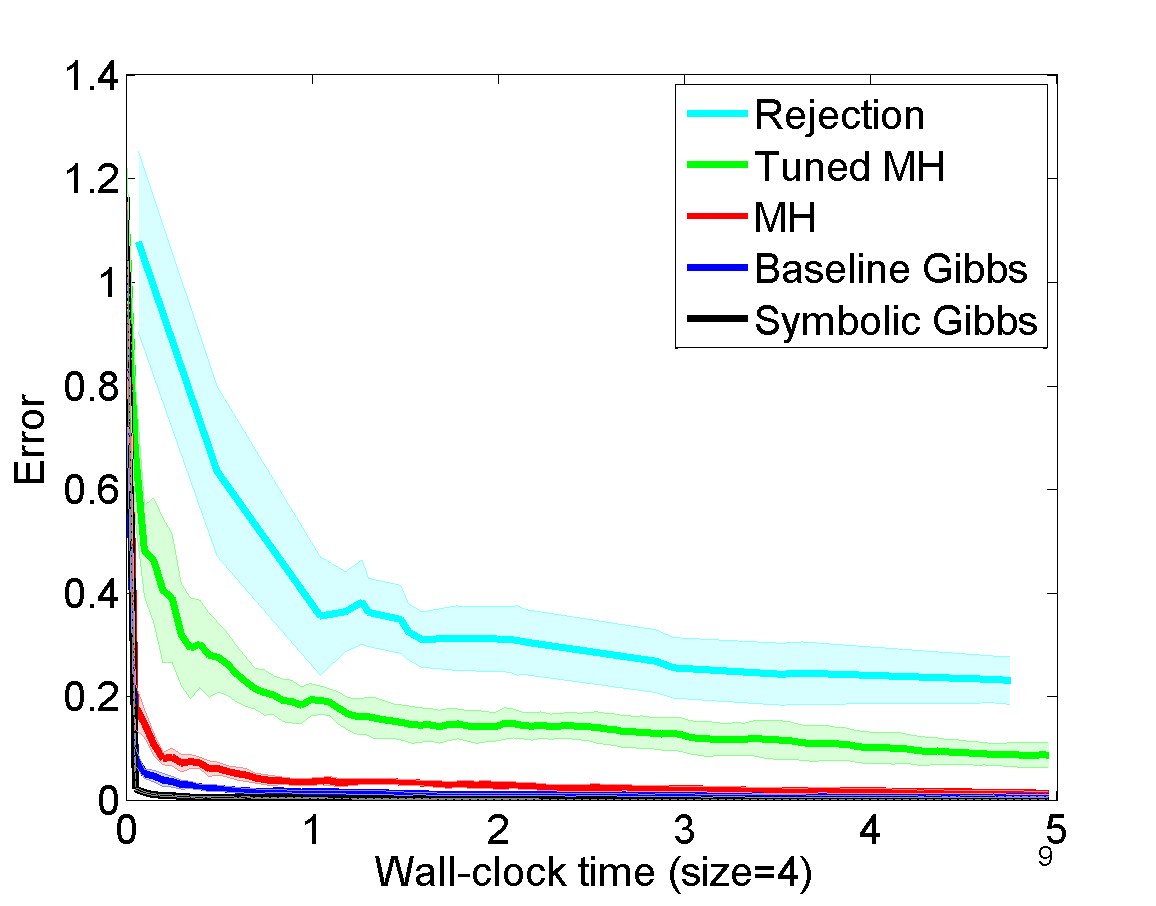
\includegraphics[width=1\linewidth, height=120pt]
{Figs/plots/collision/err-vs-time__param4-shaded.pdf}
     \caption{}
\label{fig:collision-err-vs-time4}
\end{minipage}
%%%
\begin{minipage}[b]{0.33\textwidth}
     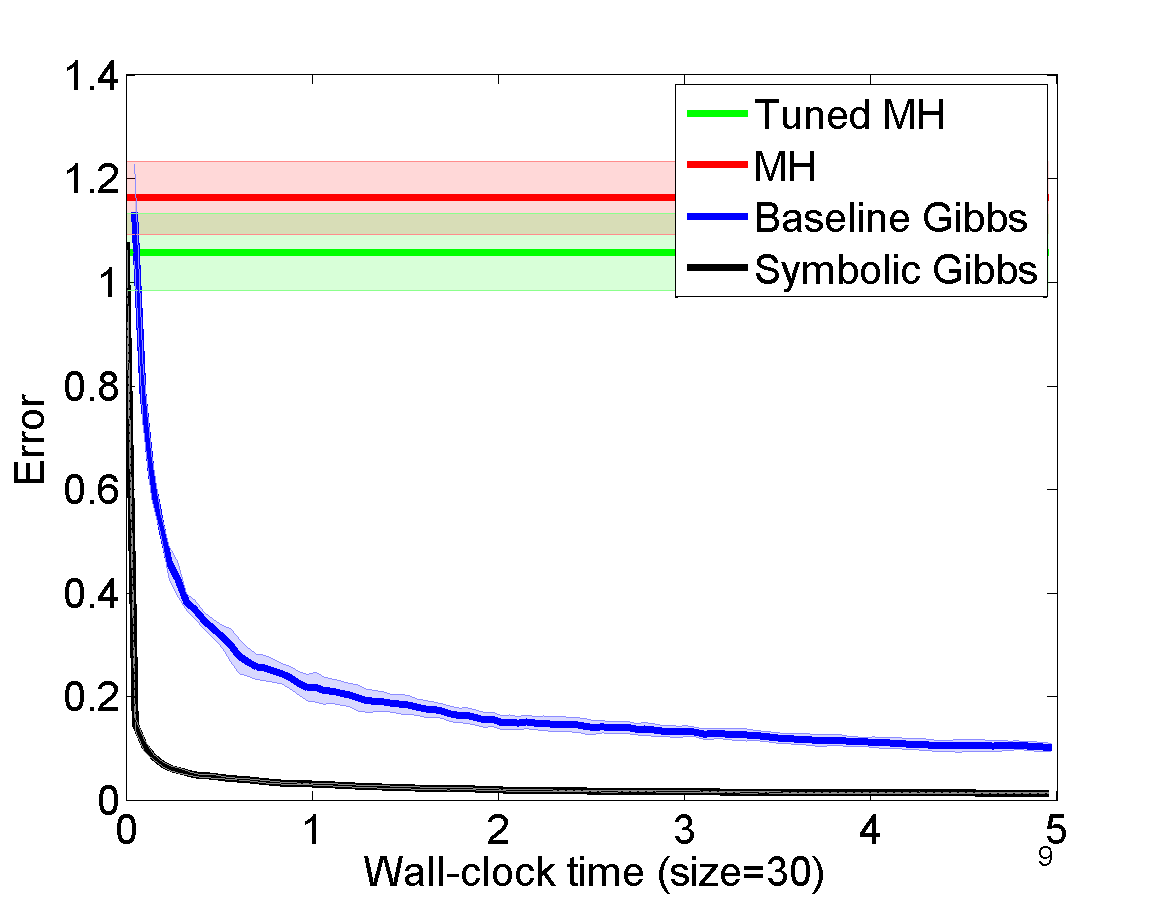
\includegraphics[width=1\linewidth, height=120pt]
{Figs/plots/collision/err-vs-time__param30-shaded.pdf}
     \caption{}
\label{fig:collision-err-vs-time30}
%\vspace{-1mm}
\end{minipage}
\begin{minipage}[b]{0.33\textwidth}
      \caption{Error %(expected value of the difference between estimated mean vector and the ground truth vector) 
as a function of wall clock time (ns) for the generalized collision problem (Experiment 2) 
(a) for 4 colliding objects (8 stochastic variables in total since each object has a distribution over its mass and its velocity) and (b) 30 colliding objects (60 stochastic variables)
using different MCs. Note that in (b), rejection sampling has not been able to take any sample.}
      \label{fig:dummy}
    \end{minipage}
\end{figure*}
%%%%%%%%%%%%%%%%%%%%%%%%%%%%%%%%%%%%%%%%%%%%%%%%%%%%%%%%
\begin{figure*}
\begin{center}
%\vspace{-1mm}
\begin{minipage}[b]{0.33\textwidth}
 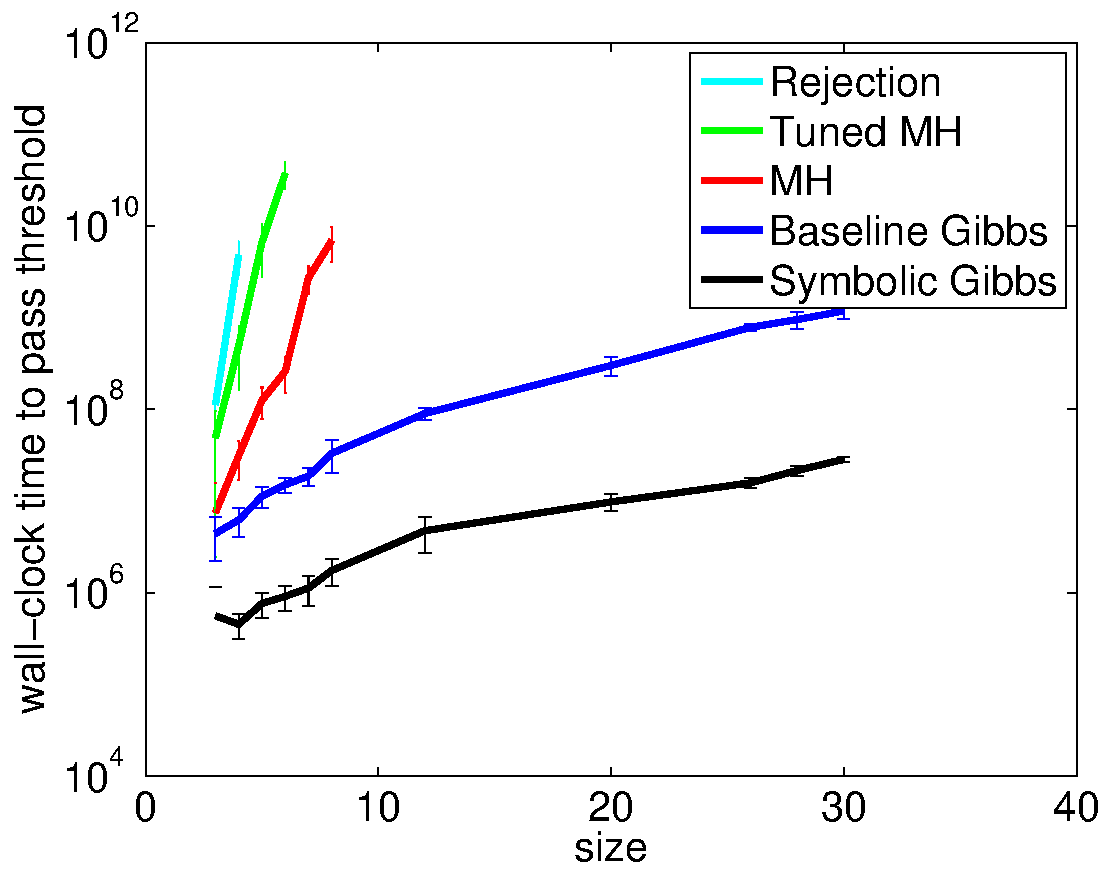
\includegraphics[width=1\linewidth, height=120pt]{Figs/plots/collision/time_vs_param-errorbar.pdf}
\caption{generalized collision problem}
\label{fig:err-threshold-vs-size-collision}
\end{minipage}
%
\begin{minipage}[b]{0.33\textwidth}
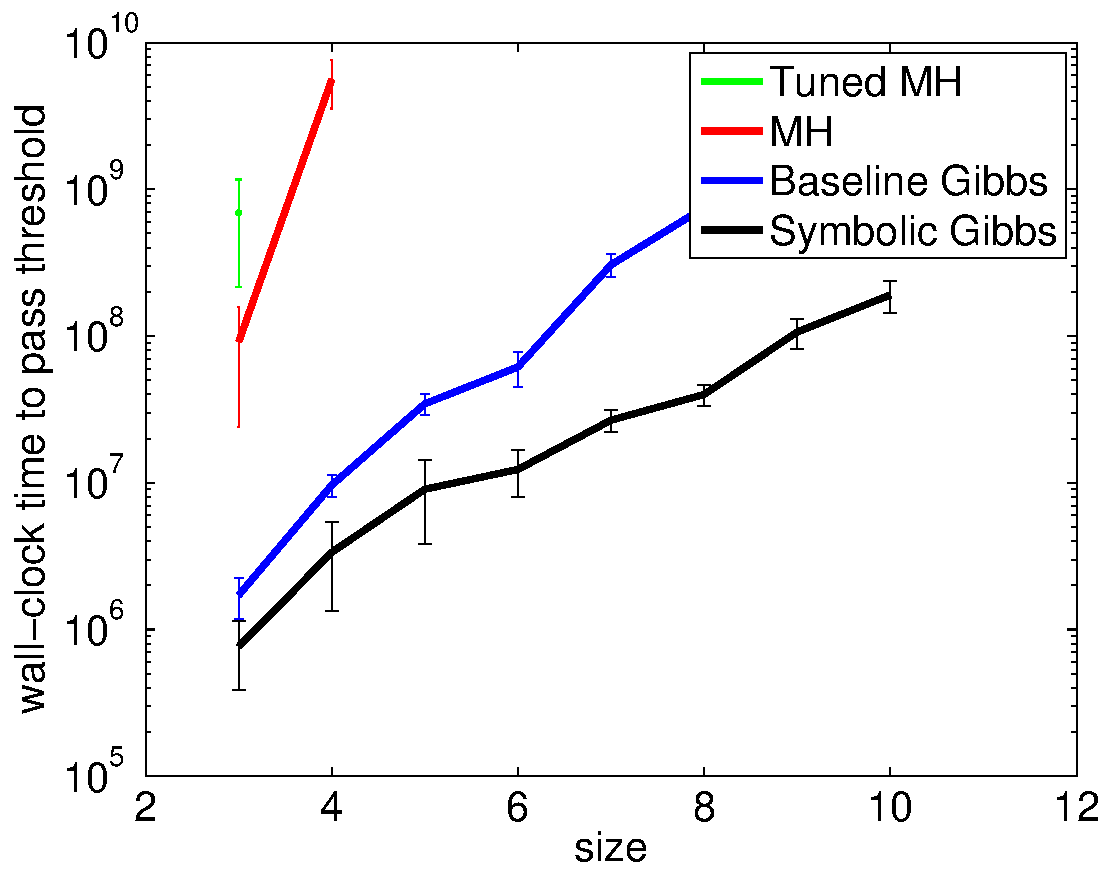
\includegraphics[width=1\linewidth, height=120pt]{Figs/plots/fermentation/time_vs_param-errorbar.pdf}
\caption{power transmission line problem}
\label{fig:err-threshold-vs-size-alc}
\end{minipage}
\begin{minipage}[b]{0.33\textwidth}
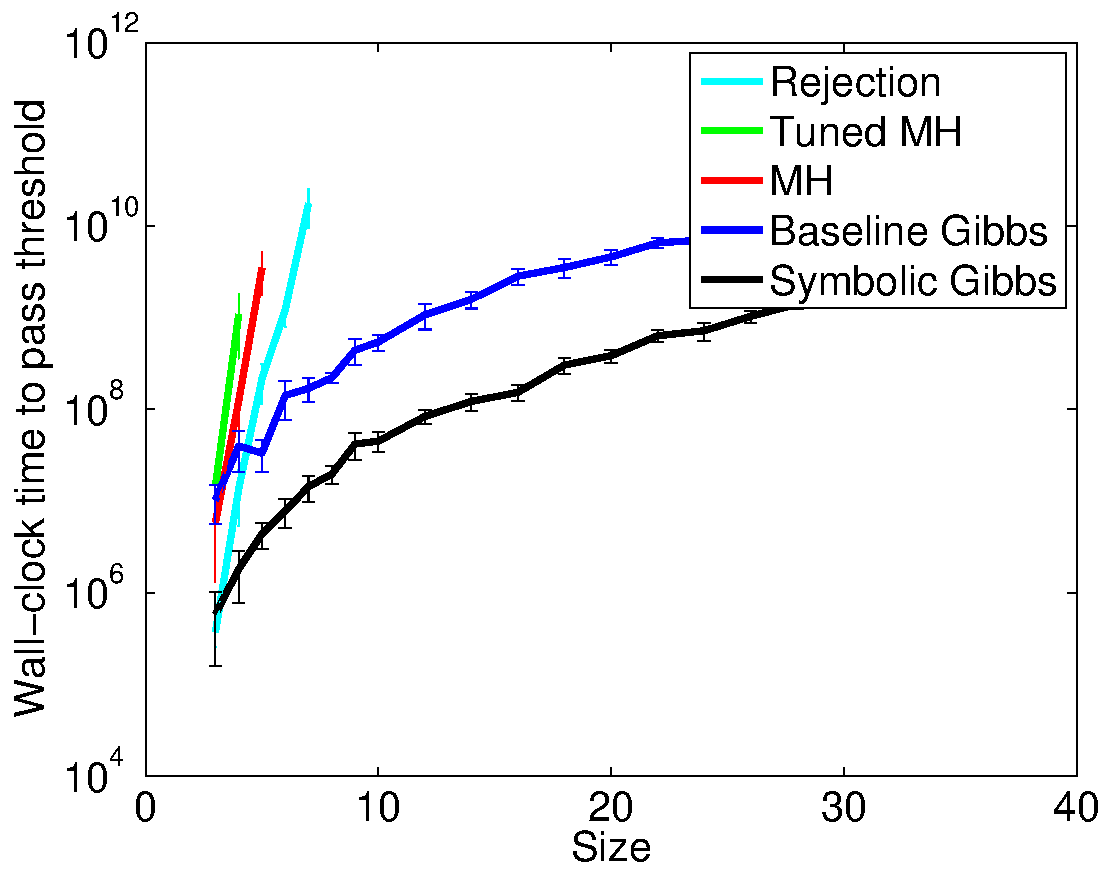
\includegraphics[width=1\linewidth, height=120pt]{Figs/plots/circuits/time_vs_param-errorbar.pdf}
\caption{reduced mass problem}
\label{fig:err-threshold-vs-size-circuit}
\end{minipage}
\end{center}
\caption{Wall-clock time (ns) to pass a fixed error threshold vs. the GM size, for experiments 2 to 4.}
\end{figure*}

%%%%%%%%%%%%%%%%%%%%%%%%%%%%%%%%%%%%%%%%%%%%%%%%%%%%%%%%
%%%%%%%%%%%%%%%%%%%%%%%%%%%%%%%%%%%%%%%%%%%%%%%%%%%%%%%%

\section{Experimental Results}
\textbf{Experiment 1.} In our first experiment, we generate samples for the GM of the \emph{collision} example and 
plot the particles for different queries and evidence.\footnote{We have repeated the experiment for different 
MCMC methods and have made sure they generate same patterns.}
The results, as depicted in the telltale plots of Figure~\ref{fig:mom}, reveal the nature of the problem tackled in this paper.
They show that even in the presence of a single deterministic constraint, 
a simple prior can transform into a complicated posterior which is unlike any family of 
probability densities studied in the literature so far.

In the second to fourth experiments, we study the role of the size of graphical model on the performance of MCMC methods.
\\
\textbf{Experiment 2.} The second experiment is the generalization of the collision example to a case where $n$ objects 
collide. The difference is that we omit the dependency of velocities (all $V_i$ share a same uniform prior distribution) and the constraint is $\sum_i{M_i V_i} = P$. By this modification, the GM becomes symmetric and enables us to compute the true posterior mean value manually.\footnote{An alternative would be relying on \emph{MCMC convergence diagnostics} methods \cite{cowles1996markov}. The latter methods however, could produce misleading results in case MCMCs do not converge to the ground truth, a scenario that for highly complex posteriors is not improbable.} 
The tested algorithms running on the posterior are: symbolic Gibbs (ours), baseline Gibbs (CDF computation per sample), 
MH (Metropolis-Hastings tuned manually), Tuned-MH 
(automatically tuned to reach the acceptance rate of 0.234 after \cite{roberts1997weak}) and rejection sampling.
For error measure, $\mathbb{E}[|\bvec{x} - \bvec{x}^*|]$ is computed in which 
$\bvec{x}^*$ is the ground truth vector.
For each algorithm 15 Markov chains run and means and standard errors are returned.     
Figures~\ref{fig:collision-err-vs-time4} 
and 
\ref{fig:collision-err-vs-time30} 
depict error vs wall-clock time in (ns) %TODO CHECK TIME SCALE!
for a collision network of 4 and 30 objects, respectively. %(the actual number of stochastic nodes is 8 since each object is associated with a mass and velocity node).
%Figure~\ref{fig:collision-err-vs-time30} depicts the same results for 30 objects (60 nodes).
In the latter high-dimensional space, the rejection sampling has not been able to generate a particle.
MH algorithms convergence rate is very low while the baseline Gibbs still perform well and the symbolic Gibbs performance is at least an order of magnitude better.
Finally, Figure~\ref{fig:err-threshold-vs-size-collision} depicts the time to reach a fixed error threshold $T=0.2$ 
versus number of colliding objects. 
%
\\
\textbf{Experiment 3.} Here, we repeat the former experiment for a 
monotonically decreasing \emph{Dynamic Bayesian Network}. That is, a DBN with nodes $A_1$ to $A_n$
with priors: $A_1 \sim \mathcal{U}(0, b)$ and $A_t \sim \mathcal{U}(A_{t-1}, b)$ where 
$t = 2, \ldots n$ and $b=10$ is the upper bound and the deterministic constraint is $\sum A_i = c$.
This network models a power transmission line where energy loss takes place in components $A_t$.
However, many other applications, such as development of a chemical process, share similar models.  
The measurement takes place on the difference of the expected values of two parallel Markov chains to form a symmetry with ground truth \textbf{0}.
In the plotted results (Figure~\ref{fig:err-threshold-vs-size-alc}), 
the rejection sampling MC is missing since the joint is not log-concave and does not have a constant bound required for the algorithm's \emph{envelope} 
(note that $\lim_{A_{i} \rightarrow b} \frac{1}{b - A_{i}} = 0$ ).
\\
\textbf{Experiment 4.} The last experiment, with results depicted in 
Figure~\ref{fig:err-threshold-vs-size-circuit}, models an electrical circuit composed of $n$, $10\Omega\pm20\%$ paralleled resistors with bell-shaped tolerance distributions (truncated quadratics, positive in the range $[8, 12]$). The posterior tolerance distribution is computed when 
the input current $I$ and the source voltage $V$ and observed and the deterministic constraint is $\frac{1}{R_1} + \ldots + \frac{1}{R_n} = \frac{I}{V}$.
This form of equation, called \emph{reduced mass}, encounters in many problems in electrical, thermal, hydraulic, or mechanical domains. 

\section{Conclusion}

We introduced piecewise algebraic graphical models that for the first time handle a large family of nonlinear deterministic restrictions, such as the physical laws, in the form of multivariate polynomial fractions. The nonlinear nature of this data leads to a new genre of posterior distributions with possible discontinuities, 
piecewise parts with nonlinear bordering hyperplanes, rapid density changes and anomalies. Our experimental results show that Gibbs sampling performs well in the presence of such unconventional densities while other Monte Carlo methods do not. We showed that in piecewise algebraic models, the univariate CDFs required for Gibbs sampling can be computed analytically and prior to the actual sampling process. Our novel sampling method, \emph{Symbolic Gibbs}, saves a significant amount of computation, improving the performance dramatically. The combination of these novel contributions should make probabilistic reasoning applicable to variety of new applications that have remained unsolvable so far.      


%*********************************************************************************************
%*********************************************************************************************
%*********************************************************************************************

% Note use of \abovespace and \belowspace to get reasonable spacing 
% above and below tabular lines. 

%\begin{table}[t]
%\caption{Classification accuracies for naive Bayes and flexible 
%Bayes on various data sets.}
%\label{sample-table}
%\vskip 0.15in
%\begin{center}
%\begin{small}
%\begin{sc}
%\begin{tabular}{lcccr}
%\hline
%\abovespace\belowspace
%Data set & Naive & Flexible & Better? \\
%\hline
%\abovespace
%Breast    & 95.9$\pm$ 0.2& 96.7$\pm$ 0.2& $\surd$ \\
%Cleveland & 83.3$\pm$ 0.6& 80.0$\pm$ 0.6& $\times$\\
%Glass2    & 61.9$\pm$ 1.4& 83.8$\pm$ 0.7& $\surd$ \\
%Credit    & 74.8$\pm$ 0.5& 78.3$\pm$ 0.6&         \\
%Horse     & 73.3$\pm$ 0.9& 69.7$\pm$ 1.0& $\times$\\
%Meta      & 67.1$\pm$ 0.6& 76.5$\pm$ 0.5& $\surd$ \\
%Pima      & 75.1$\pm$ 0.6& 73.9$\pm$ 0.5&         \\
%\belowspace
%Vehicle   & 44.9$\pm$ 0.6& 61.5$\pm$ 0.4& $\surd$ \\
%\hline
%\end{tabular}
%\end{sc}
%\end{small}
%\end{center}
%\vskip -0.1in
%\end{table}


% Acknowledgements should only appear in the accepted version. 

% In the unusual situation where you want a paper to appear in the
% references without citing it in the main text, use \nocite
%\nocite{langley00}

\bibliography{symbolic_gibbs_icml}
\bibliographystyle{icml2015}

\end{document} 


% This document was modified from the file originally made available by
% Pat Langley and Andrea Danyluk for ICML-2K. This version was
% created by Lise Getoor and Tobias Scheffer, it was slightly modified  
% from the 2010 version by Thorsten Joachims & Johannes Fuernkranz, 
% slightly modified from the 2009 version by Kiri Wagstaff and 
% Sam Roweis's 2008 version, which is slightly modified from 
% Prasad Tadepalli's 2007 version which is a lightly 
% changed version of the previous year's version by Andrew Moore, 
% which was in turn edited from those of Kristian Kersting and 
% Codrina Lauth. Alex Smola contributed to the algorithmic style files.  
